
\begin{frame}{Galat Pembulatan (\textit{Round-off Error})}

Galat pembulatan disebabkan karena komputer hanya dapat menyimpan bilangan penting
yang terbatas selamat perhitungan.

Bilangan-bilangan seperti $\pi$, $e$, dan $\sqrt{7}$ tidak dapat dinyatakan
dalam bilangan penting yang berhingga.
Bilangan-bilangan seperti $1/3 = 0.333333\ldots$ juga harus disimpan dalam digit
yang berhingga (kecuali jika disimpan dalam bentuk tipe data khusus yang dapat merepresentasikan
\emph{bilangan rasional}).

Galat pembulatan berhubungan langsung dengan bagaimana cara suatu bilangan
disimpan pada komputer. Untuk membahas ini, kita perlu mengingat kembali
mengani \emph{sistem bilangan}

\end{frame}


\begin{frame}{Sistem bilangan}

Sistem bilangan adalah suatu konvensi untuk merepresentasikan bilangan.
Untuk manusia, yang paling natural digunakan adalah \emph{sistem desimal} atau
basis-10. Pada sistem ini ada 10 digit: 0-9. Setiap digit memiliki nilai tempat.
Contoh:
$$
86409 = (8 \times 10^4) + (6 \times 10^3) + (4 \times 10^2) + (0 \times 10^1) +
(9\times 10^0)
$$

Komputer menggunakan basis-2 untuk merepresentasikan bilangan atau sistem biner.
Pada sistem ini hanya ada dua digit, yaitu 0 dan 1.
Contohnya bilangan biner $101.1_{2}$ sama dengan:
\begin{equation*}
1 \times 2^2 + 0 \times 2^1 + 1 \times 2^0 + 1 \times 2^{-1} = 4 + 0 + 1 + 0.5 = 5.5_{10}
\end{equation*}
Biasanya notasi basis pada $5.5_{10}$ tidak ditampilkan, hanya ditulis $5.5$.

\end{frame}



\begin{frame}{Sistem bilangan}

{\centering
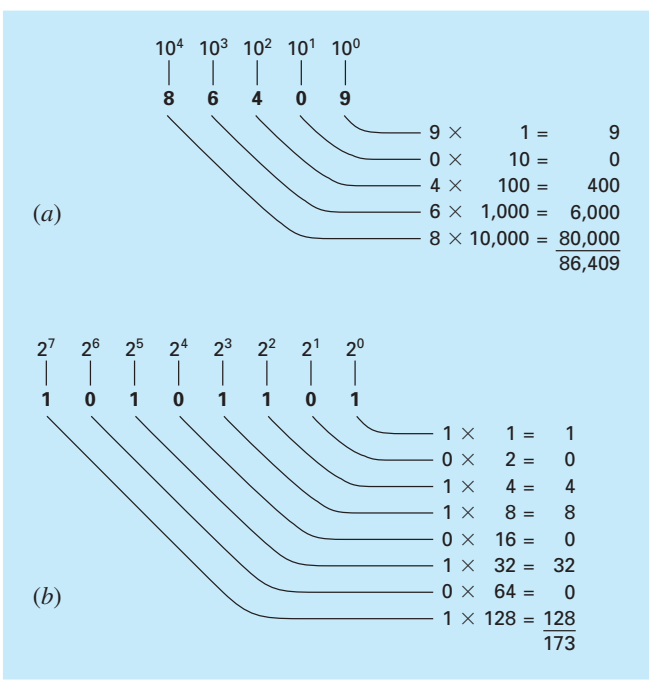
\includegraphics[height=0.8\textheight]{../chapra_7th/Chapra_Fig_3_5.png}
\par}

\end{frame}


\begin{frame}{Representasi bilangan bulat (integer)}

Metode magnitudo bertanda, \textit{signed magnitude method}, digunakan pada komputer
untuk merepresentasikan suatu bilangan. Bit pertama digunakan untuk menyatakan tanda
(0 untuk bilangan positif dan 1 untuk bilangan negatif).
Bit yang lain digunakan untuk menyimpan magnitudo bilangan.
Misalnya bilangan -173 pada komputer dengan 16-bit

{\centering
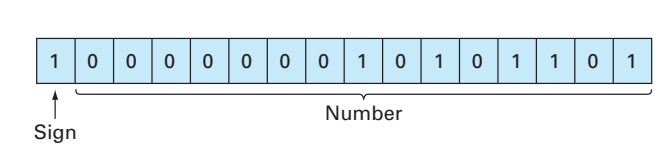
\includegraphics[height=0.3\textheight]{../chapra_7th/Chapra_Fig_3_6.png}
\par}

\end{frame}


\begin{frame}{Contoh representasi bilangan bulat}

Tentukan bilangan bulat dalam basis-10 yang dapat direpresentasikan dalam 16-bit.

Dari 16 bit yang tersedia, bit pertama digunakan menyimpan tanda.
15 bit yang tersisa dapat digunakan untuk menyimpan bilangan biner
dari 0 sampai 111111111111111 yang sama dengan
$$
(1 \times 2^{14}) + (1 \times 2^{13}) + \cdots +
(1 \times 2^{1}) + (1 \times 2^{0}) = 32767
$$
Oleh karena itu 16 bit dapat digunakan untuk merepresentasikan bilangan bulat
dari -32767 sampai 32767
Bilangan 0 sudah didefinisikan sebagai 0000000000000000, maka
1000000000000000 tidak perlu digunakan untuk menyatakan minus 0. Oleh karena itu
biasanya representasi biner tersebut digunakan untuk mereprentasikan bilangan
negatif tambahan, yaitu -32768.

\end{frame}



\begin{frame}[fragile]{Metode komplemen-2}

Pada komputer modern, metode magnitudo bertanda yang dijelaskan sebelumnya
tidak secara langsung digunakan. Metode alternatif (namun masih terkait)
yaitu metode komplemen-2 (\textit{2's complement}) digunakan. Pada metode ini
kita tidak memerlukan bit khusus untuk menyimpan tanda.

Misalnya kita ingin menyatakan bilangan -28 pada komputer 8-bit.
Pertama angka 28 dinyatakan dalam bilangan biner, yaitu:
\begin{textcode}
00011100
\end{textcode}
Untuk menyatakan angka -28, pertama kita inversi bilangan biner tersebut
(0 menjadi 1, 1 menjadi 0):
\begin{textcode}
11100011
\end{textcode}
kemudian tambahkan 1:
\begin{textcode}
11100100
\end{textcode}

\end{frame}


\begin{frame}{\textit{Overflow} dan \textit{underflow}}

Detil mengenai representasi bilangan pada komputer tidak menjadi fokus dalam
kuliah ini, namun pesan yang ingin disampaikan adalah \textbf{adanya
limitasi jika kita merepresentasi bilangan bulat pada komputer dengan
jumlah bit yang terbatas}.

Tipe bilangan bulat yang sering digunakan adalah \texttt{Int32} (menggunakan
32 bit) dan \texttt{Int64} (menggunakan 64 bit). Beberapa bahasa pemrograman juga
mendukung \texttt{Int16} dan \texttt{Int8}.
Untuk tiap tipe bilangan bulat atau integer tersebut, ada nilai terbesar
dan terkecil yang dapat direpresentasikan.

Jika operasi perhitungan yang kita lakukan menghasilkan
bilangan bulat yang lebih besar dari rentang nilai yang mungkin
maka yang terjadi adalah \textit{overflow}

Jika operasi perhitungan yang kita lakukan menghasilkan
bilangan bulat yang lebih kecil dari rentang nilai yang mungkin
maka yang terjadi adalah \textit{underflow}

\end{frame}




\begin{frame}[fragile]{Catatan khusus untuk Python}

Pada Python kita tidak perlu mendeklarasikan terlebih dahulu suatu variabel memiliki
suatu tipe tertentu. Tipe suatu variabel pada Python dapat berubah-ubah (dinamis), dan
biasanya secara \textit{default} dapat terjadi konversi tipe secara \textit{implisit} (otomatis, tidak
perlu diperintahkan oleh \textit{programmer} atau pengguna).

Sebagai demonstrasi, coba perhatikan keluaran dari kode ini:
\begin{pythoncode}
a = 2
type(a) # int
# Ubah variabel a
a = a + 1.1
type(a) # float
\end{pythoncode}

\end{frame}



\begin{frame}[fragile]{Catatan khusus untuk Python}

Tipe data integer \textit{default} pada Python bukanlah tipe integer yang umum.
\pyinline{int} pada Python merupakan tipe bilangan bulat khusus yang dirancang agar dapat
memiliki lebar bit yang adaptif, sehingga tidak memungkinkan terjadinya
\textit{overflow} maupun \textit{underflow}.

Tipe data \texttt{Int32} dan \texttt{Int64} (dan juga beberapa tipe data dengan lebar bit
tetap) dapat kita akses melalui pustaka Numpy. Pada pustaka Numpy, tipe-tipe data
tersebut dapat diakses dengan menggunakan \pyinline{np.int32} dan \pyinline{np.int64}.
Numpy juga menyediakan tipe data \pyinline{np.int8} dan \pyinline{np.int16}.
Fungsi \pyinline{np.iinfo()} dapat digunakan untuk mengetahui nilai terbesar
dan terkecil yang mungkin untuk setiap tipe data tersebut.

\begin{pythoncode}
import numpy as np
np.iinfo(np.int16)
\end{pythoncode}

\end{frame}




\begin{frame}[fragile]{Contoh Python}

Fungsi \pyinline{type} dapat digunakan untuk mengetahui tipe dari suatu
variabel.

\begin{pythoncode}
import numpy as np
a = np.int8(127) # variabel a dengan tipe np.int8
b = np.int8(a + 1) # berapa nilai b? Seharusnya ini akan menghasilkan overflow
type(a), type(b)
# TUGAS: Coba lakukan operasi yang menghasilkan underflow
\end{pythoncode}

Pada kode berikut ini Python akan melakukan konversi ke tipe dengan lebar bit
yang lebih besar.
\begin{pythoncode}
a = np.int(127)
b = a + 1
type(a), type(b) # sekarang apakah tipe dari b?
\end{pythoncode}

\end{frame}


\begin{frame}{Representasi bilangan titik-mengambang (\textit{floating point})}

Kuantitas numerik dengan pecahan dan yang memiliki digit di belakang koma,
biasanya direpresentasikan
pada komputer dengan menggunakan format bilangan titik-mengambang atau sering disebut sebagai
\textit{floating-point number}. Pada pendekatan ini, suatu bilangan dinyatakan sebagai:
\begin{equation*}
\pm s \times b^{e}
\end{equation*}
dengan $s$ adalah \emph{significand} atau \emph{mantissa}, $b$ adalah \emph{basis} dari sistem
bilangan yang digunakan, dan $e$ adalah eksponen.

Pada komputer basis yang digunakan adalah basis-2 (biner). Tanda (\textit{sign}),
mantissa dan eksponen akan direpresentasikan dengan menggunakan basis-2 dengan
lebar bit atau jumlah digit tertentu. Semakin besar lebar bit yang digunakan semakin teliti
representasi dari bilangan.

\end{frame}


\begin{frame}{Bilangan titik mengambang}

Sebelum dinyatakan dalam bentuk ini, suatu bilangan dinormalisasi terlebih dahulu dengan cara
memindahkan titik, desimal, biner dan sebagainya sedemikian rupa sehingga hanya satu digit
yang berada di kiri tanda titik. Hal ini dilakukan untuk menghemat memori karena tidak ada
bilangan nol yang tidak signifikan yang perlu disimpan.

Contoh: bilangan 0.005678 dapat direpresentasikan tanpa normalisasi sebagai
$0.005678 \times 10^{0}$. Namun dengan normalisasi, nilai tersebut akan disimpan
sebagai $5.678 \times 10^{-3}$, artinya dua nol sebelum digit 5 tidak perlu disimpan.

Ketika kita melakukan normalisasi untuk bilangan dengan basis 2, digit yang berada di kiri tanda
titik biner akan selalu bernilai 1.

\end{frame}


\begin{frame}{Implikasi dari representasi \textit{floating point}}
\fontsize{9}{10}\selectfont

Anggap kita memiliki "komputer" hipotetik basis-10 dengan unit penyimpan angka
yang terdiri dari 5 digit. Asumsikan bahwa satu digit
akan digunakan sebagai tanda, dua untuk eksponen, dan dua untuk mantissa.
Asumsikan juga satu digit dari eksponen digunakan untuk menyimpan tanda, dan satu digit lagi
untuk besar dari eksponen.
$$
s_1 d_1 d_2 \times 10^{s_0 d_0}
$$
$s_0$: tanda untuk eksponen dan $s_1$: tanda untuk mantissa.
$d_0$: magnitudo dari eksponen dan $d_1, d_2$: magnitudo dari mantissa.

Angka terbesar yang dapat direpresentasikan adalah
$+9.9 \times 10^{+9}$ sedangkan angka terkecilnya adalah $-1.0 \times 10^{-9}$

{\centering
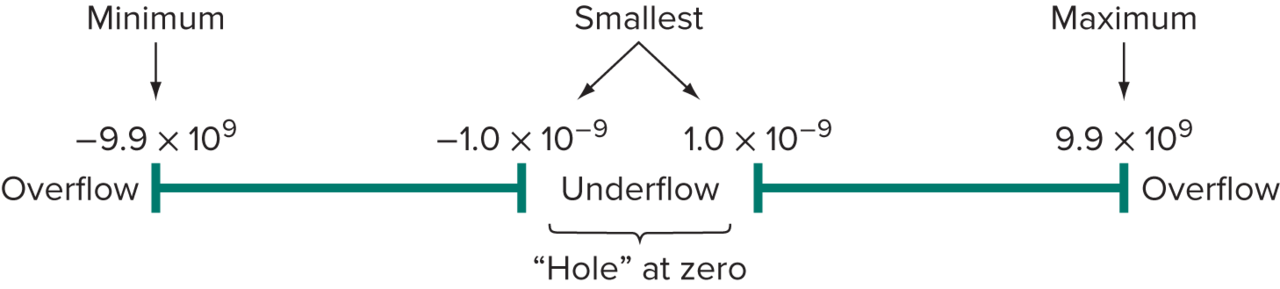
\includegraphics[height=0.25\textheight]{../chapra_python/Chapra_Fig_4_4.png}
\par}

Mirip dengan representasi bilangan integer, \emph{overflow error} dan
\emph{underflow error} juga dapat terjadi.


\end{frame}




\begin{frame}
\fontsize{9}{9}\selectfont

Pada komputer ini, bilangan seperti $2^{-5} = 0.03125$ terpaksa harus disimpan sebagai
$3.1\times 10^{-2}$. Pada saat inilah \emph{galat pembulatan} terjadi.
Untuk kasus ini kita dapat menghitung galat ini sebesar:
$$
\frac{0.03125 - 0.031}{0.03125}\times 100\% = 0.8\%
$$
Kita dapat mengurangi galat ini dengan cara menambah digit mantissa.

Bilangan lain, misalnya bilangan irasional seperti $\pi$ harus disimpan sebagai
$3.1\times 10^{0}$ dan galatnya adalah:
$$
\frac{3.14159\ldots - 3.1}{3.14159\ldots} \times 100\% \approx 1.32\%
$$
Penambahan digit mantissa dapat mengurangi galat ini, namun galat ini tidak akan pernah
bernilai nol karena bilangan irasional memiliki jumlah digit yang tak hingga.

\end{frame}


\begin{frame}

Pada gambar berikut, bilangan yang dapat dinyatakan secara eksak ditampilkan sebagai garis
vertikal pendek. Bilangan-bilangan lainnya akan mengalami galat pembulatan.

{\centering
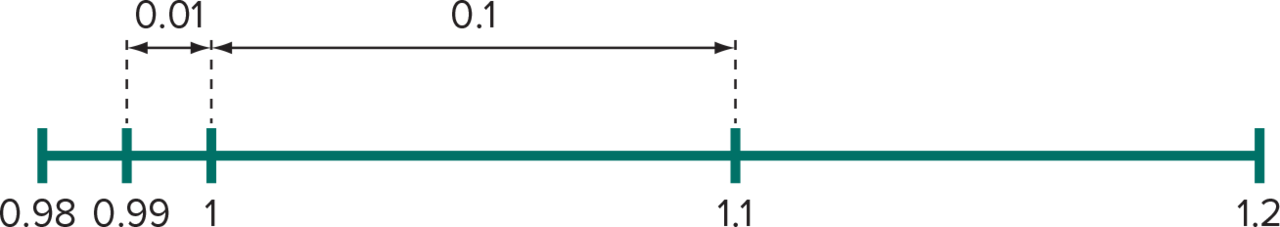
\includegraphics[height=0.2\textheight]{../chapra_python/Chapra_Fig_4_5.png}
\par}

Chopping vs rounding

\end{frame}


\begin{frame}{\textit{Machine epsilon}}

Perhatikan bahwa celah atau jarak antar bilangan akan meningkat ketika kita berpindah dari
satu orde magnitudo ke orde magnitudo yang lain. Misalnya untuk bilangan dengan
eksponen -1, yaitu antara 0.1 dan 1, jarak antar bilangan adalah 0.01. Ketika kita melewati
satu orde magnitudo, yaitu dari 1 sampai 10, celah ini meningkat ke 0.1. Hal ini berarti bahwa
galat pembulatan dari suatu bilangan akan sebanding dengan magnitudonya. Selain itu, hal ini
juga berarti bahwa galat relatif akan memiliki batas atas. Pada contoh sebelumnya (komputer
hipotetik dengan basis 10), galat relatif maksimum adalah 0.05. Nilai ini sering
juga disebut sebagai epsilon mesin (\textit{machine epsilon})
atau presisi mesin (\textit{machine precision}).

Epsilon mesin dapat dihitung dari:
$$
\epsilon = b^{1-t}
$$
dengan $b$ adalah basis, dan $t$ jumlah digit signifikan pada mantissa.

\end{frame}


\begin{frame}{IEEE 754}

Tipe bilangan titik mengambang yang sering digunakan adalah \textit{double-precision
floating point} yang dijelaskan dalam standard IEEE 754. Pada standard ini digunakan
64 bit.

{\centering
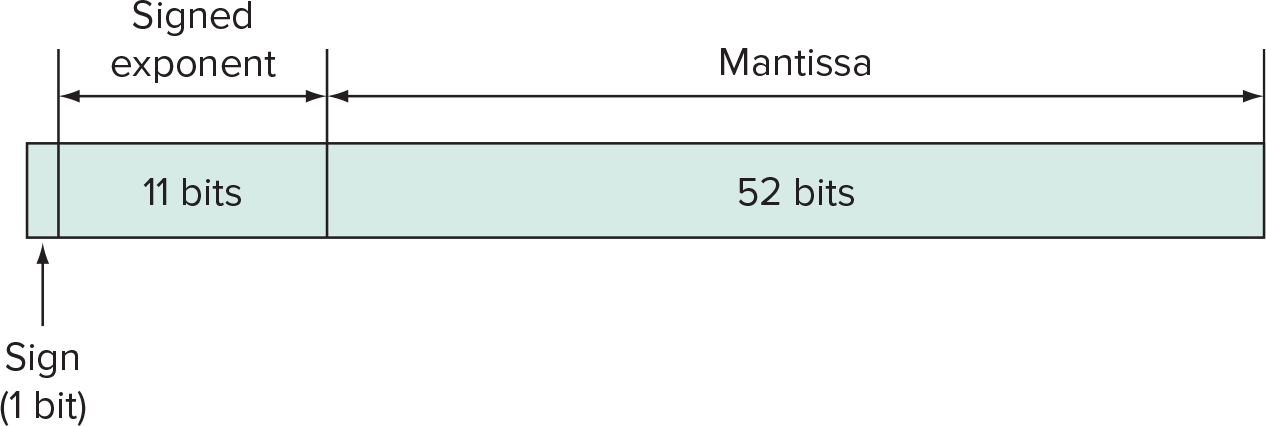
\includegraphics[height=0.25\textheight]{../chapra_python/Chapra_Fig_4_6.png}
\par}

Tipe lainnya yang juga dapat digunakan adalah \textit{single-precision} (32 bit),
\textit{half-precision} (16 bit), dan \textit{quadruple-precision} (128 bit).

\end{frame}



\begin{frame}{Python}

np.finfo(np.float64)

Contoh perhitungan: penjumlahan, rumus kuadrat, perhitungan $e^{10}$
dan $e^{-10}$, perbandingan dengan 0.

\end{frame}

